\section{Beskrivende dataanalyse (5 poeng)}\label{beskrivende-dataanalyse-5-poeng}
Datasettet består av totalt 2906 observasjoner. For analysen, så har vi valgt å fokusere de følgende variablene; pris (realSum), avstand til sentrum (dist), kapasitet (person\textunderscore capacity) og tilfredsstillhet (guest\textunderscore satisfaction\textunderscore overall), da det er disse variablene som er mest relevant for våre problemstillinger.

En gjennomgang av datasettet, viser at gjenomsnittsprisen for en natt for to personer, en helg i Lisboa er 240 euro, medianprisen er noe lavere på 227. Et høyere gjennomsnitt indikerer en noe høyreskev fordeling. Det er en håndful dyrere utleieboliger som drar opp prisen. Leilighetene ligger i snitt ganske nært sentrum, med en avstand på 1.97km, og gjestene er generelt svært fornøyde med en median på 93/100 for gjestetilfredstillhet. 


\paragraph{Prisfordeling} \mbox{} \\
Ettersom at pris er hovedfokuset i regresjonsanalysen, har vi undersøkt fordelingen ved bruk av histogram. Fordelingen av av \textbf{realSum} bekrefter observasjonen om høyreskjevhet. Den største andelen av leilighetene koster under 300  euro, mens den lange "halen" som strekker seg mot høyre er de få dyrere og mer ekslusive leilighetene.

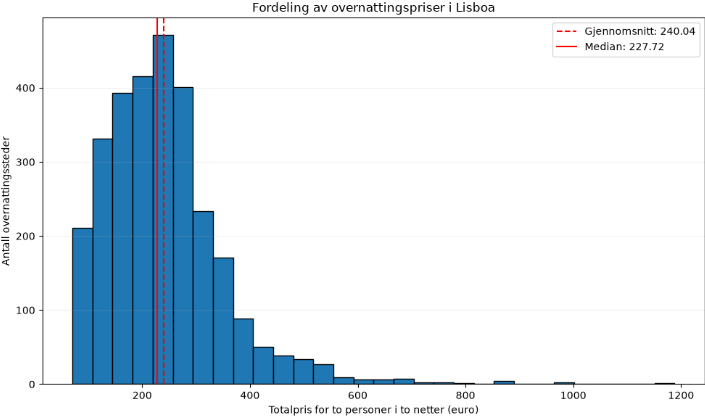
\includegraphics[]{Images/fordeling_overnattingspriser.png}

Her bør du gjennomføre en kort deskriptiv dataanalyse for å få en
oversikt over datasettet. Det betyr at man lager noen visualiseringer
for å forstå dataene bedre, og at man beregner noen enkle ting. Fokuser
på det som er relevant for modelleringen, og bruk sunn fornuft. For mye
detaljer eller figurer uten forklaring og tydelige akseetiketter er ikke
nyttige for leseren.

\paragraph{Sammenhenger} \mbox{}\\
Vi har benyttet spredningsdiagram som å undersøke sammenhengen mellom pris og beliggenhet. Diagrammet viser at leilighetene som ligger nærmest sentrum har både den høyeste gjennomsnittsprisen og størst variasjon og pris.

Variabelen \textbf{person\textunderscore capacity} har som forventet høyest korrelasjon med pris på (r = 0.567). Avstand til sentrum (\textbf{dist}) har overraskende nok en negativ korrelasjon på (r = -0.146), og gjestefilfredstillhet har en positiv korrelasjon på (r = 0.148).


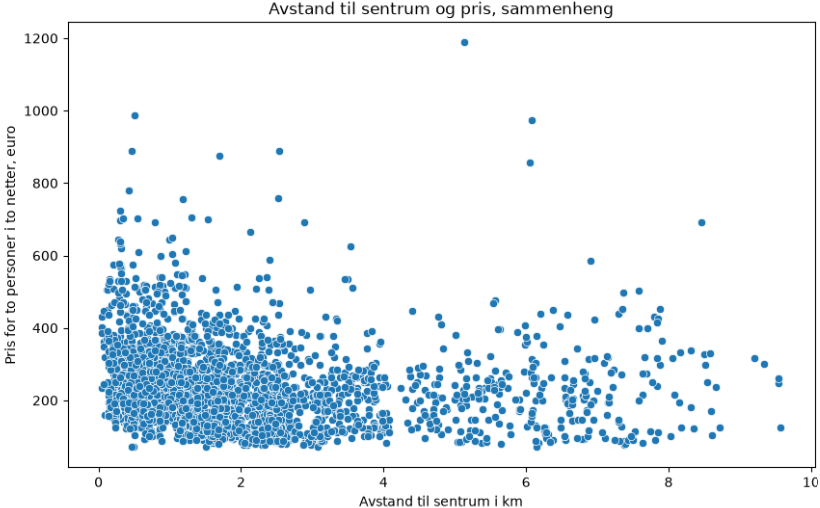
\includegraphics[]{Images/avstand_til_sentrum_pris_sammenheng.png}

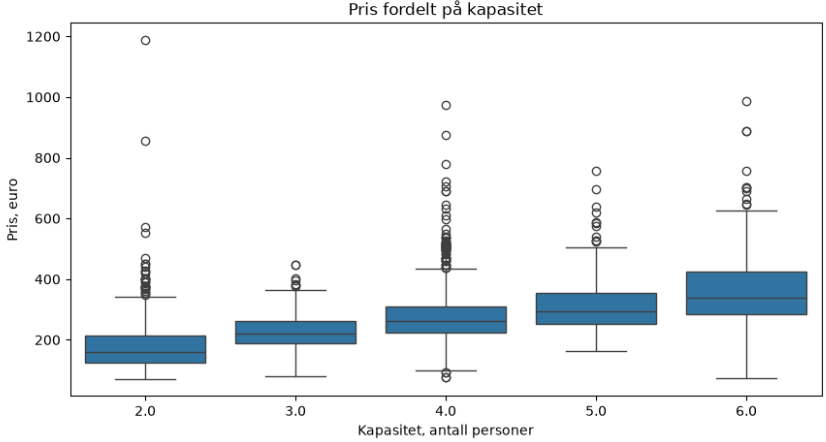
\includegraphics[]{Images/boksplott_pris_gruppert_kapasitet.png}

Du kan for eksempel:

\begin{itemize}
\tightlist
\item
  Presentere deskriptiv statistikk, som gjennomsnitt, median,
  standardavvik og varians, for å beskrive datasettets sentraltendens,
  variasjon og fordeling.
\item
  Bruke spredningsdiagrammer (scatter plots) og korrelasjonsmatriser for
  å undersøke sammenhenger mellom ulike variabler.
\item
  Bruke histogrammer for å vise fordelingen til relevante variabler.
\item
  Bruke boksplott (box plots) for å undersøke fordeling, variasjon og
  eventuelle uteliggere.
\end{itemize}

Resultatene bør forklares i teksten, med særlig fokus på funn som kan
være relevante for den videre modelleringen. Skriv en kort legende under
hver grafikk, slik at det blir tydelig hva grafikken viser.